%% ---------------------------------------------------------------------------
\section{Experimental Setup}
\label{sec:setup}

\paragraph{Real trajectories.} We use the public SWE-agent trajectories submitted
to the SWE-bench Lite leaderboard~\citep{jimenez2024swebench,yang2024sweagent}
by five LLMs spanning two interface generations: GPT-4, Claude~3 Opus and GPT-4o
with the SWE-agent 0.x interface, and Claude~3.7 Sonnet and Claude~4 Sonnet with
SWE-agent 1.x (1{,}478 trajectories in total; \cref{tab:corpus}). Each
trajectory is parsed into a system turn, the task (issue text), and alternating
agent and tool turns; state writes are derived from actions as described in
\cref{sec:method} and \cref{app:probes}. For each trajectory and budget
$B\in\{4\text{k},8\text{k},16\text{k}\}$ tokens we evaluate up to six decision
points whose uncompressed history exceeds $B$ (7{,}949 / 6{,}227 / 4{,}572
decision points), probing every key written so far (125k / 119k / 114k state
probes per compressor) and every eligible identifier in the next action (40k /
37k / 31k use probes).

\paragraph{\textsc{StateTrack}.} The synthetic benchmark generates agent-like
trajectories with three key families: \emph{pinned} constraints stated in the
task and occasionally revised by the user ($p=0.004$ per key and step),
\emph{slow} facts rewritten rarely ($p=0.03$), and \emph{fast} status variables
rewritten often ($p=0.25$). Writes appear as \texttt{key = value} lines inside
tool outputs (80\%) or agent notes (20\%), surrounded by log-like distractor
lines (lognormal, mean 25 lines per output). Values are unique, so the ideal
reader is exact. Unless stated otherwise we use 150 steps, 4 pinned, 12 slow and
6 fast keys, 30 seeds, and probe all keys at three checkpoints.

\paragraph{Compressors.} We compare SKC and SKC+BM25 with five model-free
baselines covering the main families used in practice (settings in
\cref{app:settings}): \textbf{recency window} (FIFO truncation with the task
pinned), \textbf{observation masking}~\citep{lindenbauer2025complexity},
\textbf{truncate observations} (cap each older tool output), \textbf{BM25
selection} (salience-based selection, a turn-level stand-in for
importance-pruning methods~\citep{li2023selective,jiang2023llmlingua}), and
\textbf{random selection}. We do not include LLM summarization, which
requires running an LLM over every prefix; see \cref{sec:limitations}.

\begin{table}[t]
\centering
\small
\caption{SWE-agent trajectories used in this study (SWE-bench Lite). Tokens are
counted over task, agent and tool turns of the full trajectory. ``Far
$>$10'': fraction of identifiers used in an action that first appeared more than
10 steps earlier.}
\label{tab:corpus}
\begin{tabular}{lrrrrrrr}
\toprule
Model (interface) & Traj. & \multicolumn{2}{c}{Steps} & \multicolumn{2}{c}{Tokens} & Tool & Far \\
 & & median & p90 & median & p90 & share & $>$10 \\
\midrule
GPT-4 (0.x)            & 300 & 20 & 34 & 13.1k & 24.7k & 79\% & 33\% \\
Claude 3 Opus (0.x)    & 300 & 18 & 23 &  7.9k & 11.8k & 82\% & 21\% \\
GPT-4o (0.x)           & 278 & 40 & 65 & 22.6k & 49.5k & 89\% & 67\% \\
Claude 3.7 Sonnet (1.x)& 300 & 29 & 54 & 27.3k & 51.6k & 81\% & 61\% \\
Claude 4 Sonnet (1.x)  & 300 & 59 & 91 & 34.7k & 56.7k & 71\% & 79\% \\
\bottomrule
\end{tabular}
\end{table}

%% ---------------------------------------------------------------------------
\section{Results}
\label{sec:results}

\subsection{What long agent contexts are made of}
\label{sec:corpus}

\Cref{tab:corpus} and \cref{fig:corpus} characterize the trajectories. Tool
outputs make up 71--89\% of all tokens. Newer models run longer and reach
further back: for Claude~4 Sonnet the median trajectory has 59 steps and 35k
tokens, and 79\% of the identifiers its actions use first appeared more than
ten steps earlier (21\% for Claude~3 Opus). State writes split into command
outputs (35\%), file views (33\%), edits (27\%) and searches (5\%); a median
trajectory rewrites 4--7 keys at least once. Long horizons therefore come with
both long-range dependencies and frequent overwrites---exactly the two
conditions under which our analysis predicts that windows lose state and
selection produces stale state.

\begin{figure}[t]
\centering
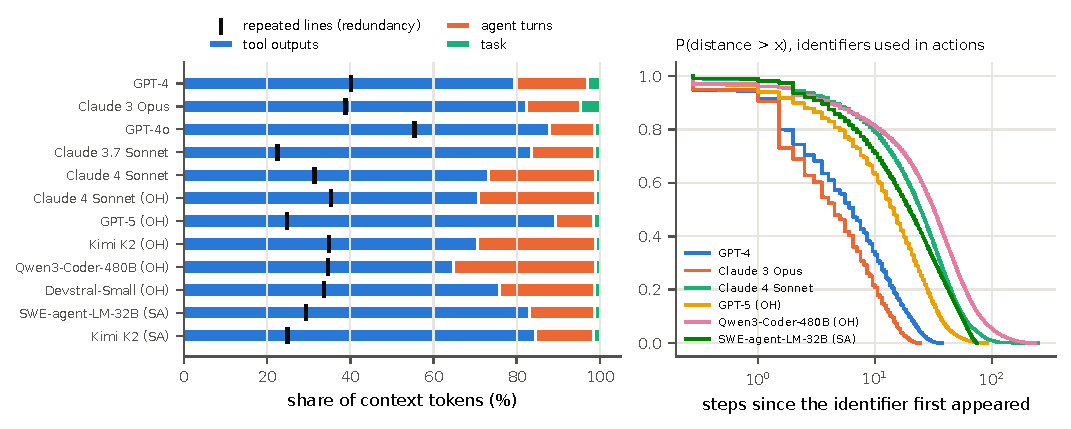
\includegraphics[width=\linewidth]{figures/corpus.pdf}
\caption{Left: share of context tokens by turn type. Right: survival function of
the distance (in steps) between an identifier's first occurrence and its use in
an action.}
\label{fig:corpus}
\end{figure}

\subsection{Main results on real trajectories}
\label{sec:main}

\begin{table}[t]
\centering
\small
\caption{Real SWE-agent trajectories, pooled over five models. State probes: \%
correct and \% stale (the rest are missing). Use probes: \% of identifiers used
by the next action that are still available; ``long'': those last seen more
than two steps earlier. Best in \textbf{bold}.}
\label{tab:main}
\setlength{\tabcolsep}{4pt}
\begin{tabular}{l rrr rrr rrr}
\toprule
 & \multicolumn{3}{c}{State correct $\uparrow$} & \multicolumn{3}{c}{State stale $\downarrow$} & \multicolumn{3}{c}{Use (long) available $\uparrow$} \\
\cmidrule(lr){2-4}\cmidrule(lr){5-7}\cmidrule(lr){8-10}
Compressor & 4k & 8k & 16k & 4k & 8k & 16k & 4k & 8k & 16k \\
\midrule
Recency window        & 40.0 & 52.0 & 66.1 & 0.3 & 0.2 & \textbf{0.1} & 63.0 & 82.9 & 92.8 \\
Observation masking   & 38.8 & 43.1 & 39.0 & 0.3 & 0.3 & 0.6 & 63.3 & 81.5 & 88.7 \\
Truncate observations & 43.1 & 52.5 & 62.1 & 0.6 & 1.0 & 1.3 & 70.3 & 84.5 & 90.2 \\
BM25 selection        & 39.4 & 46.8 & 58.3 & 1.6 & 1.7 & 1.7 & \textbf{76.4} & \textbf{89.9} & 95.2 \\
Random selection      & 51.8 & 63.6 & 75.5 & 2.4 & 1.9 & 1.2 & 71.4 & 84.7 & 93.6 \\
\midrule
SKC (ours)            & \textbf{66.2} & 76.4 & 83.0 & \textbf{0.1} & \textbf{0.1} & \textbf{0.1} & 71.1 & 83.4 & 93.1 \\
SKC+BM25 (ours)       & 66.1 & \textbf{76.7} & \textbf{83.1} & 0.4 & 0.3 & 0.3 & 72.2 & 88.2 & \textbf{95.6} \\
\bottomrule
\end{tabular}
\end{table}

\begin{figure}[t]
\centering
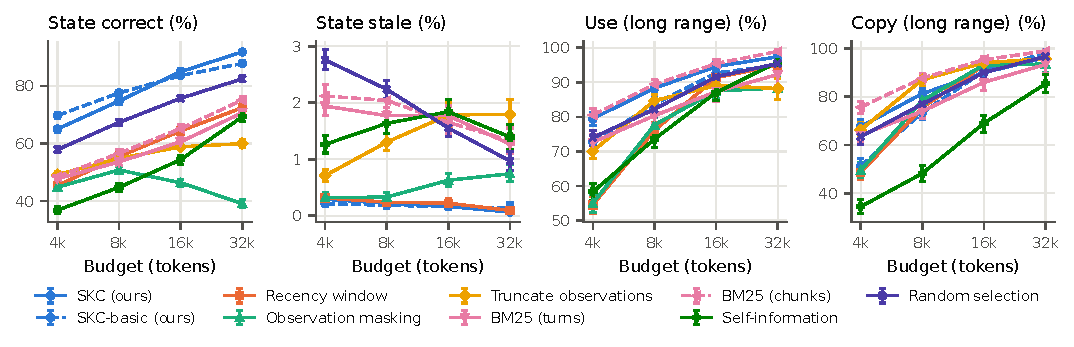
\includegraphics[width=\linewidth]{figures/real_budget.pdf}
\caption{Real trajectories, pooled over five models, as a function of the budget.}
\label{fig:real-budget}
\end{figure}

\paragraph{State retention.} \Cref{tab:main} and \cref{fig:real-budget}
summarize the main comparison. At every budget SKC retains far more of the
agent's state than any baseline: 66\% / 76\% / 83\% of state probes are
correct at 4k / 8k / 16k tokens, versus 40\% / 52\% / 66\% for the recency
window and 39\% / 43\% / 39\% for observation masking. The gain holds for each
of the five models (\cref{tab:by-model} in the appendix): at 8k, SKC improves
over the best non-random baseline by 12 (Claude~3 Opus) to 27 (Claude~4
Sonnet) points, and is within 2 points of or above every baseline for every
model. Random selection is the strongest baseline on this metric because it
spreads the budget over the whole history, but it pays for it in staleness
(below).

\paragraph{Staleness.} Supersession-blind selection leaves stale state:
BM25 and random selection are stale on 1.2--2.4\% of all probes, 12--24 times
more than SKC (0.1\%). The aggregate hides the dependence on overwrites
predicted by \cref{prop:stale}: among keys written three or more times, 9--11\%
of BM25 and random probes are stale, i.e.\ 10--16\% of the values these
methods retain for such keys are outdated (\cref{fig:stale-real}). Recency
windows and observation masking, which are (nearly) supersession-consistent,
stay at or below 2.3\% even for frequently rewritten keys; residual staleness comes
from truncated turns and from edits whose evidence is only partially kept.

\begin{figure}[t]
\centering
\begin{minipage}{0.37\linewidth}
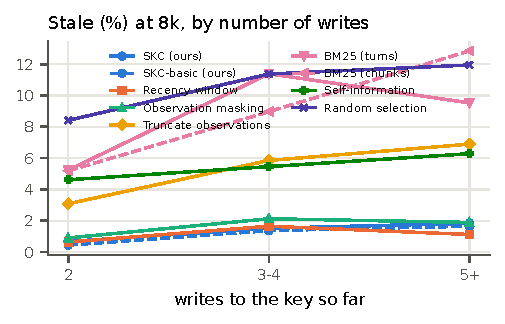
\includegraphics[width=\linewidth]{figures/real_stale_nwrites.pdf}
\end{minipage}\hfill
\begin{minipage}{0.6\linewidth}
\caption{Stale rate on real trajectories (8k) by the number of writes the key
has received. Selection methods (BM25, random) approach the regime predicted by
\cref{prop:stale}; supersession-consistent methods stay low. Keys written once
cannot be stale.}
\label{fig:stale-real}
\end{minipage}
\end{figure}

\paragraph{Forgetting by age.} \Cref{fig:real-age} (left) breaks state probes
down by the age of the key's latest write. Recency windows and observation
masking are as good as SKC for keys written in the last five steps and
collapse beyond ten: for keys last written 21--40 steps ago, 14\% (window) and
10\% (masking) are retained, versus 70\% for SKC, which degrades gracefully
(58\% beyond 40 steps). This is \cref{prop:window} in action: windows forget by
age, regardless of importance.

\begin{figure}[t]
\centering
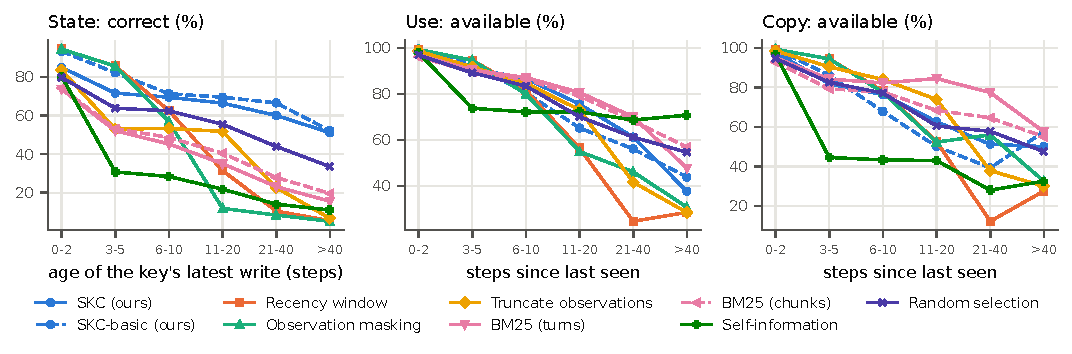
\includegraphics[width=\linewidth]{figures/real_age.pdf}
\caption{Real trajectories at 8k. Left: state probes by the age of the key's
latest write. Right: use probes by the number of steps since the identifier
last appeared.}
\label{fig:real-age}
\end{figure}

\paragraph{Per key family.} \Cref{tab:by-family} shows where the gains come
from. SKC retains 87\% of command outputs and 92\% of search results at 8k
(window: 50\% and 41\%), because these are small, high-value records once the
long outputs around them are dropped. Edits improve from 50--57\% to 75\%. File
views are the exception: they are large (often a 100-line window), have the
lowest priority, and are cut by the value cap, so SKC retains 52\% of them,
below random selection (64\%). This is a deliberate trade-off of the default
priority, analysed further in the ablations.

\begin{table}[t]
\centering
\small
\caption{Real trajectories at 8k: \% correct by key family (and \% stale for
the mutable families). The task is pinned by every method. Probe counts: edit
24.5k, view 32.0k, cmd 47.9k, search 8.5k, task 6.2k.}
\label{tab:by-family}
\setlength{\tabcolsep}{4pt}
\begin{tabular}{l rrrrr rrrr}
\toprule
 & \multicolumn{5}{c}{Correct (\%)} & \multicolumn{4}{c}{Stale (\%)} \\
\cmidrule(lr){2-6}\cmidrule(lr){7-10}
Compressor & task & edit & view & cmd & search & edit & view & cmd & search \\
\midrule
Recency window        & 100 & 50.2 & 49.3 & 50.3 & 40.9 & 0.6 & 0.2 & 0.1 & 0.0 \\
Observation masking   & 100 & 51.6 & 38.9 & 35.7 & 33.7 & 0.9 & 0.5 & 0.1 & 0.0 \\
Truncate observations & 100 & 56.7 & 28.9 & 56.9 & 69.0 & 1.3 & 1.5 & 0.8 & 0.2 \\
BM25 selection        & 100 & 56.3 & 50.8 & 35.0 & 31.4 & 2.1 & 2.7 & 1.3 & 0.3 \\
Random selection      & 100 & 56.2 & \textbf{63.9} & 61.2 & 70.5 & 2.4 & 2.8 & 1.6 & 0.4 \\
\midrule
SKC (ours)            & 100 & 75.4 & 52.0 & \textbf{87.4} & \textbf{91.6} & 0.2 & 0.3 & 0.0 & 0.0 \\
SKC+BM25 (ours)       & 100 & \textbf{75.7} & 53.6 & 87.0 & 91.1 & 0.2 & 0.8 & 0.1 & 0.0 \\
\bottomrule
\end{tabular}
\end{table}

\paragraph{Use probes: does compression remove what the agent uses next?}
Use probes do not depend on our key definitions. For identifiers that occurred
in the last two steps every method is near 100\%, so we focus on long-range
use probes (\cref{tab:main}, right; \cref{fig:real-age}, right). Here the
picture is different from the state probes: BM25 selection is the best single
method (76\% at 4k, 90\% at 8k), because its query includes the latest agent
turn, which is lexically close to the next action. SKC improves on the window
and on masking (71\% vs.\ 63\% at 4k) but not on BM25. SKC+BM25, which spends
the leftover budget on relevance, closes most of that gap (72\% / 88\% / 96\%)
while keeping SKC's state retention and a stale rate of 0.3\%, five times
lower than BM25's. In other words, the ledger and relevance-based selection
are complementary: the ledger guarantees that the current value of each key is
present (and, by \cref{cor:safe}, that the selected older turns cannot make it
stale), and relevance recovers older context that the next step is likely to
need.

\subsection{Controlled experiments on \textsc{StateTrack}}
\label{sec:synthetic}

\begin{figure}[t]
\centering
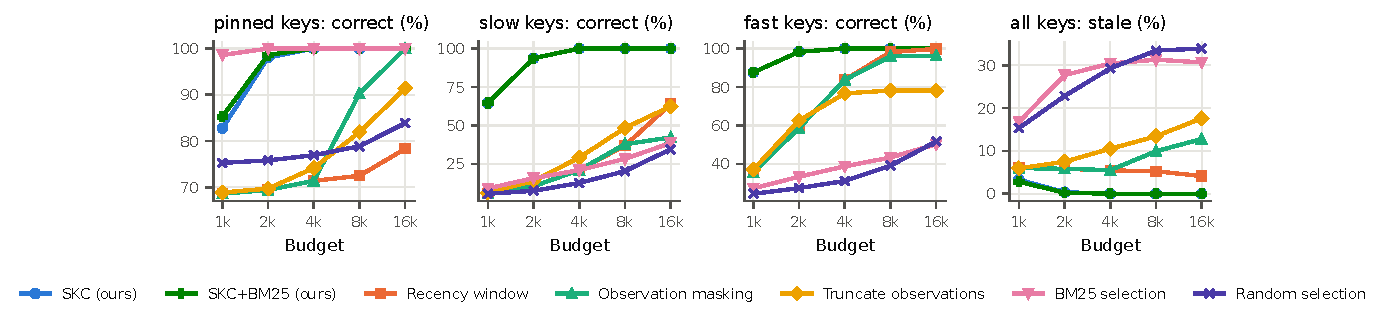
\includegraphics[width=\linewidth]{figures/synth_budget.pdf}
\caption{\textsc{StateTrack} (30 seeds): \% correct per key family and \%
stale over all keys, as a function of the budget. SKC and SKC+BM25 overlap.}
\label{fig:synth-budget}
\end{figure}

\paragraph{Budget and key families.} \Cref{fig:synth-budget} separates the
three families. Windows and masking retain fast keys once the budget covers a
few steps but lose most slow keys (at most 38\% up to 8k; window 64\% and
masking 42\% at 16k), as \cref{prop:window} predicts for small $\lambda_k$. Selection methods retain
pinned keys (their text overlaps the query) but are stale on about 30\% of all
probes from 4k up. SKC reaches 96\% correct at 2k and 100\% from 4k, with
almost no stale state. Note one subtle failure of \emph{every} baseline:
pinning the task is itself not supersession-consistent, because a user's later
revision of a pinned constraint is lost while the original stays pinned; this
accounts for the 4--6\% stale rate of the recency window.

\paragraph{Horizon.} At a fixed 4k budget (\cref{fig:synth-horizon}) the
accuracy of all baselines falls as trajectories grow from 50 to 800 steps
(window: 53\%$\to$31\%) while their stale rates grow (BM25: 24\%$\to$48\%;
window: 3\%$\to$17\%, from pinned constraints whose revisions fall out of
the window);
SKC stays at 100\%, as \cref{prop:sufficiency} predicts when the number of keys
is fixed.

\begin{figure}[t]
\centering
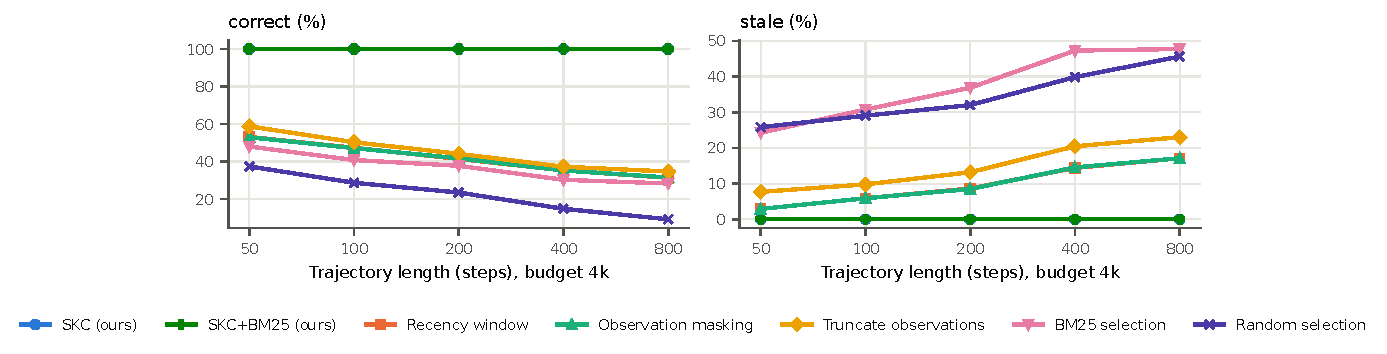
\includegraphics[width=\linewidth]{figures/synth_horizon.pdf}
\caption{\textsc{StateTrack}, budget 4k: accuracy and staleness vs.\
trajectory length. SKC and SKC+BM25 overlap at 100\% correct and 0\% stale.}
\label{fig:synth-horizon}
\end{figure}

\paragraph{Validating \cref{prop:stale}.} \Cref{fig:synth-stale} plots the
stale rate against the number of writes $m$ for random and BM25 selection,
with \cref{eq:stale} evaluated at the empirical fraction $\rho$ of turns kept.
The prediction tracks random selection closely at all three budgets; BM25 is
noisier and tends to sit above it at small budgets, because its scores are
correlated with lexical overlap rather than independent. Window and SKC are
never stale.

\begin{figure}[t]
\centering
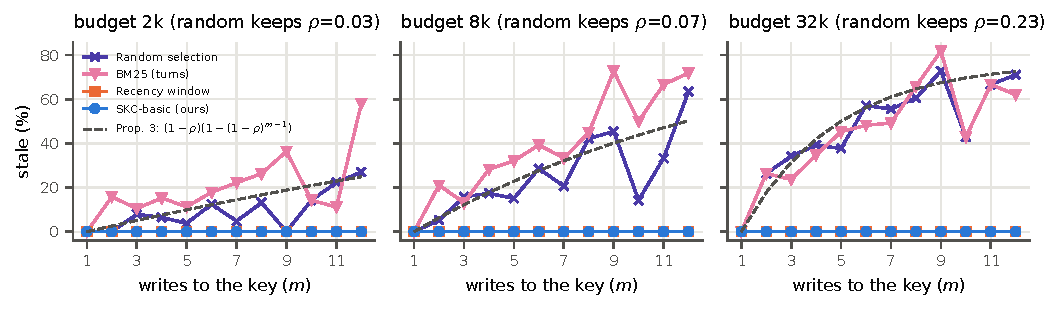
\includegraphics[width=\linewidth]{figures/synth_stale_theory.pdf}
\caption{Stale rate vs.\ number of writes per key ($m$) in \textsc{StateTrack}
(200 steps, 12 fast keys). Dashed: \cref{prop:stale} with the measured $\rho$.}
\label{fig:synth-stale}
\end{figure}

\paragraph{Imperfect extraction.} \Cref{fig:synth-recall} degrades the
extractor's recall $r$. A ledger alone (no raw window) behaves exactly as
\cref{prop:stale} predicts with $\rho=r$: at $r=0.7$, 25\% of probes are stale.
SKC's raw recent window and backward extension hedge against missed writes,
because the latest write of an actively changing key is usually recent: at 8k
and $r=0.7$, SKC is stale on 8\% of probes and correct on 88\%, against 25\% and
69\% for the ledger alone. SKC+BM25 is more exposed (16\% stale), because its
extension is supersession-blind and \cref{cor:safe} only protects keys whose
latest write the ledger actually holds. Extraction quality is therefore the
critical dependency of state-keyed methods, and when it is uncertain, the
leftover budget is better spent on a raw window than on relevance.

\begin{figure}[t]
\centering
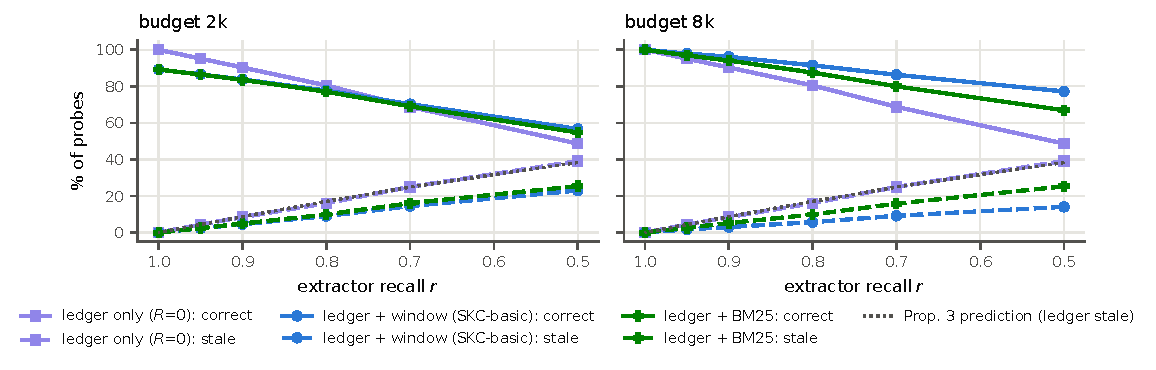
\includegraphics[width=\linewidth]{figures/synth_recall.pdf}
\caption{SKC variants under extractor recall $r$ (\textsc{StateTrack}, 30
seeds). Solid: correct; dashed: stale; dotted: \cref{prop:stale} with $\rho=r$
for the ledger alone.}
\label{fig:synth-recall}
\end{figure}

\paragraph{Capacity.} When the number of keys grows at a fixed 2k budget
(\cref{fig:synth-capacity}), SKC degrades as the ledger stops fitting (98\% at
20 keys, 64\% at 100, 28\% at 400), as the lower bound of
\cref{prop:sufficiency} requires; windows and masking fall from 29\% to 4\%.
With uniform probe probabilities and equal record sizes, every priority order
is equally good (\cref{prop:knapsack}); we verified that recency-only and FIFO
priorities match the default to within one point.

\begin{figure}[t]
\centering
\begin{minipage}{0.4\linewidth}
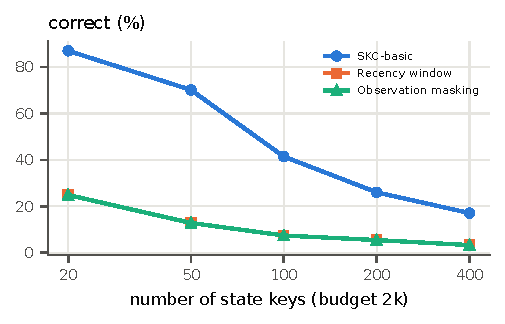
\includegraphics[width=\linewidth]{figures/synth_capacity.pdf}
\end{minipage}\hfill
\begin{minipage}{0.56\linewidth}
\caption{Retention as the number of state keys grows at a fixed 2k budget
(\textsc{StateTrack}, 200 steps). Full retention requires space linear in the
number of live keys (\cref{prop:sufficiency}); SKC degrades gracefully once the
ledger no longer fits, while windows retain only recently written keys.}
\label{fig:synth-capacity}
\end{minipage}
\end{figure}

\subsection{Ablations on real trajectories}
\label{sec:ablation}

Ablation results pending.


%% ---------------------------------------------------------------------------
\section{Discussion and Limitations}
\label{sec:limitations}

\paragraph{Sufficiency is not success.} We measure whether information is
\emph{present} for an ideal reader. Real models may fail to use information that
is present (e.g.\ in the middle of a long context~\citep{liu2024lost}) and may
recover information that is absent (by re-running a command or re-opening a
file). Our numbers are therefore upper bounds on what compression permits, not
predictions of solve rates. Measuring end-to-end task success with LLM agents
on compressed contexts is the most important next step; this study could not
call LLMs.

\paragraph{No LLM summarization baseline.} Summarization is a widely used
compressor~\citep{wang2023recursively,lindenbauer2025complexity,kang2025acon}
that we could not run. Our analysis still applies to it: a summary is
supersession-consistent only if the summarizer reliably replaces old values by
new ones, which is precisely the extraction problem of \cref{sec:synthetic},
and recursive summaries can compound such errors over time.
\citet{lindenbauer2025complexity} found that observation masking matches LLM
summarization in solve rate on SWE-bench, which suggests summarization does not
dominate the baselines we include.

\paragraph{Probe design.} State keys are derived by the same structural parser
that SKC uses, which advantages SKC on state probes. We mitigate this in three
ways: key-free use probes, a synthetic benchmark with exact ground truth, and
noisy-extractor experiments; we also report where SKC loses (file views; long
range use probes against BM25). The evidence threshold ($\theta=0.8$), the
evidence sampling, and the regular-expression token counts are design choices;
other choices change absolute numbers but not the qualitative ordering we
observed during development.

\paragraph{Domain.} Our real data come from one agent scaffold (two
generations of SWE-agent) on one task family (repository-level bug fixing).
Structural extraction is easiest when tools are typed; agents whose state
lives mostly in free text (dialogue, web browsing) need learned extractors,
whose recall then governs staleness (\cref{prop:stale}).

%% ---------------------------------------------------------------------------
\section{Conclusion}

Agent histories are event logs, and the information an agent must keep is the
current state those events define. Viewing compression through this lens
separates two failure modes---missing and stale state---and explains when
common compressors exhibit them: windows forget by age, and
supersession-blind selection retains outdated values at a rate that grows with
the number of overwrites. Log compaction is the natural remedy. A simple,
model-free implementation, SKC, retains 66--83\% of agent state on real SWE-agent
trajectories at 4k--16k tokens (vs.\ 39--66\% for windows and observation
masking) with a stale rate of 0.1\%, and its hybrid with relevance selection
also preserves the long-range information agents go on to use. The
remaining challenges are extraction for unstructured state and end-to-end
validation with LLM agents.
